\documentclass[11pt]{article}
\usepackage[margin=0.8in]{geometry}
\usepackage{multirow}
\usepackage {graphicx}
\usepackage[utf8x]{inputenc} % указать кодировку русского текста
\usepackage[russian]{babel} % указать, что язык текста - русский
\usepackage{fancyhdr}
\pagestyle{fancy}
\begin{document}
\begin{titlepage}
\begin{center}
%\vspace*{1cm}
\large\textbf{Московский Физико-Технический Институт}\\
\large\textbf{(государственный университет)}
\vfill
\line(1,0){430}\\[1mm]
\huge\textbf{Определение вязкости воздуха по скорости течения через тонкие трубки}\\
\line(1,0){430}\\[1mm]
\vfill
\large ФОПФ\\
\end{center}
\end{titlepage}
\fancyhead[L] {Работа 1.3.3}
\noindent \textbf{Цель работы:} \\
\indent Экспериментально выявить участок сформированного течения, определить режимы ламинарного и турбулентного течения; определить число Рейнольдса.


\noindent \textbf{В работе используются:} \\
\indent Металлические трубки, укрепленные на горизонтальной подставке; газовый счетчик; микроманометр типа ММН; стеклянная U-образная трубка; секундомер.
\section*{Описание работы}\
\indent Рассмотрим движение вязкой жидкости или газа по трубке круглого сечения. При малых скоростях потока движение оказывается ламинарным (слоистым), скорости частиц меняются по радиусу и направлены вдоль оси трубки. С увеличением скорости потока движение
становится турбулентным, и слои перемешиваются. При турбулентном движении скорость в каждой точке быстро меняет величину и направление, сохраняется только средняя величина скорости.

Характер движения газа (или жидкости) в трубке определяется безразмерным числом Рейнольдса: $$Re=\frac{vrp}{\eta}$$

В гладких трубах круглого сечения переход от ламинарного движения к турбулентному происходит при Re ≈ 1000.

При ламинарном течении объем газа V, протекающий за время t по трубе длиной l (называемый расходом), определяется формулой Пуазейля: $$Q_V=\frac{\pi r^4}{8l\eta}(P_1-P_2)$$
При	втекании	газа	в	
трубку	из большого резервуара скорости слоев вначале постоянны по всему сечению.
\indent По мере продвижения  газа по	трубке	
картина распределения скоростей меняется, так как сила трения о стенку тормозит прилежащие к ней слои. Характерное для ламинарного	
течения параболическое распределение скоростей устанавливается на	
некотором расстоянии a от входа в трубку, которое зависит от радиуса трубки r и числа Рейнольдса по формуле: $$a\approx0,2r*Re$$
\newpage
Экспериментальная установка:
\\
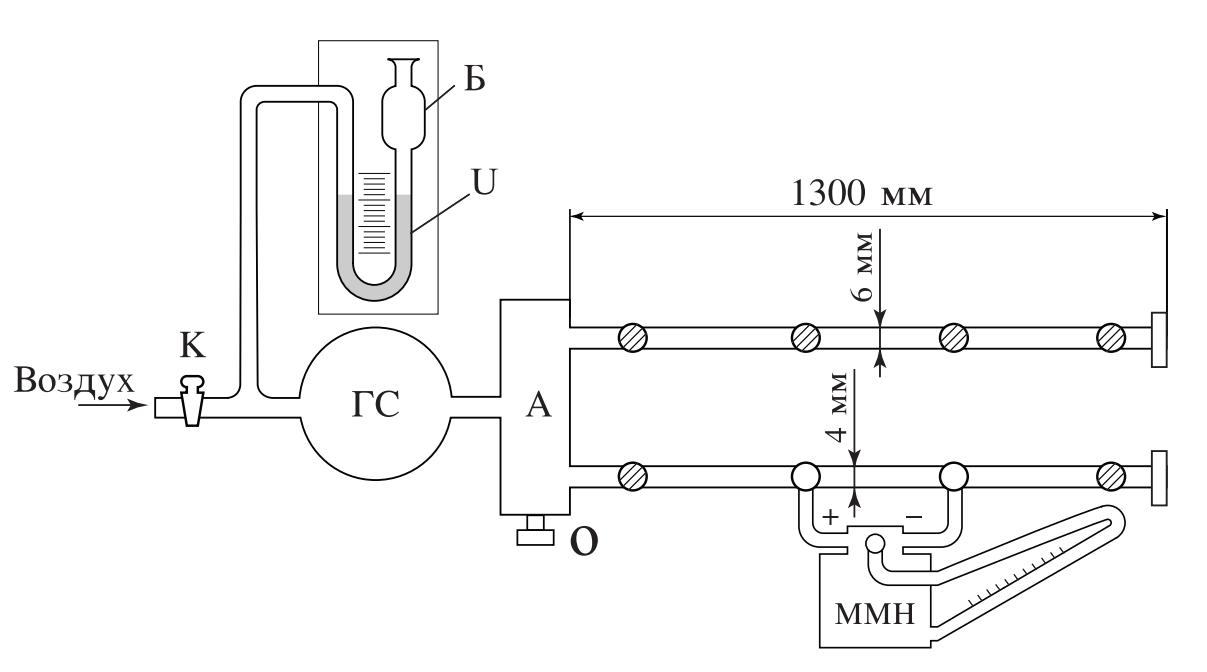
\includegraphics[scale=0.6]{asd.png} \\
А также подробная схема ММН:
\\
\ \\ \
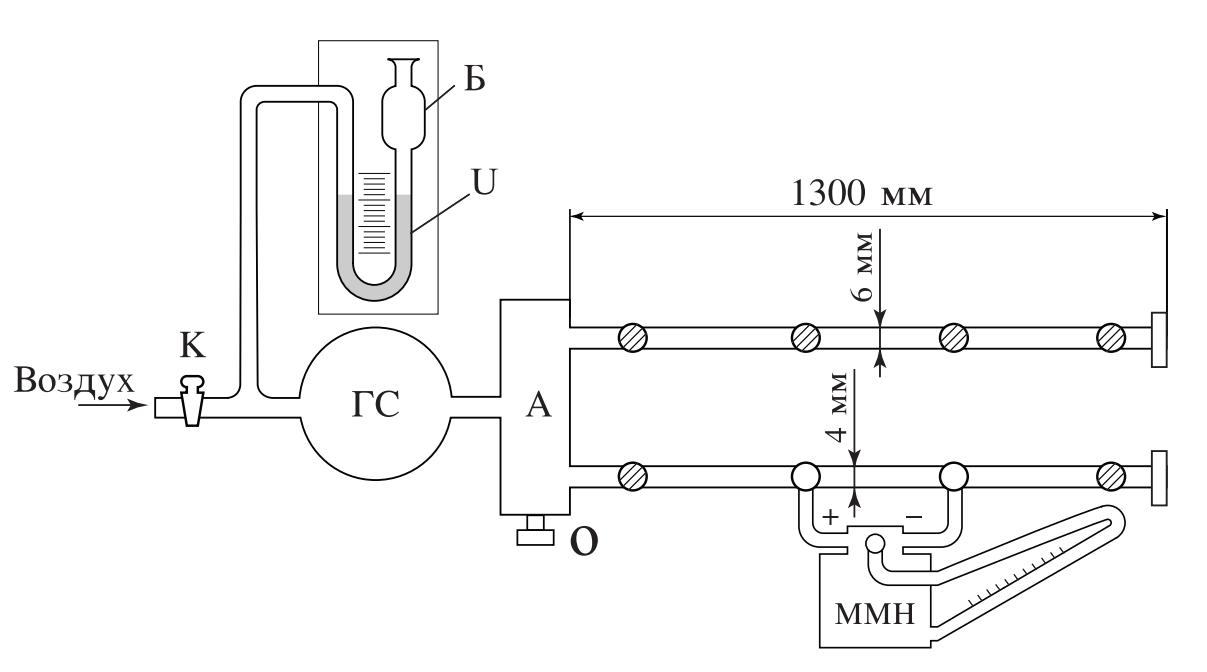
\includegraphics[scale=0.4]{asd.png}


\section*{Ход работы}\
\indent Оценим расстояние, на котором происходит формирование потока при ламинарном течении.
$a\approx0,2r*Re=0,2*1,95*10^{-2}*1000\approx 40$ (см)

Давление, измеряемое микроманометром, определяется по формуле:
$$P=K*h*9,80665$$
где \\
P - давление в Паскалях \\
$h$ отчет по шкале\\
$K=0,2$ - постоянная угла наклона\\
Таблица измерений:\\
\begin{tabular}{|c|c|c|c|c|c|c|c|c|c|c|c|c|c|c|c|c|c|}
\hline 
h, дел & 6 & 16 & 32 & 50 & 66 & 81 & 88 & 101 & 122  \\ 
\hline 
V нач, л & 2,6 & 4,6 & 0,7 & 4,0 & 0,0 & 2,5 & 2,0 & 3,0 & 2,0  \\ 
\hline 
V конеч, л & 3,5 & 6,8 & 5,1 & 8,8 & 5,5 & 8,5 & 8,5 & 10,0 & 9,0  \\ 
\hline 
t, с & 92 & 89 & 92 & 66 & 60 & 60 & 63 & 64 & 60  \\ 
\hline 
q*10$^2$, л/c & 1,0 & 2,5 & 4,8 & 7,3 & 9,2 & 10,0 & 10,3 & 10,9 & 11,7  \\ 
\hline 
\end{tabular} $\Delta h = 0,5$ дел
\ \\
\ \\
\ \\
\begin{tabular}{|c|c|c|c|c|c|c|c|c|c|c|c|c|c|c|c|c|c|}
\hline 
h, дел & 133 & 143 & 166 & 188 & 202 & 213 & 229 & 253 \\ 
\hline 
V нач, л  & 3,5 & 1,5 & 3,0 & 0,0 & 0,0 & 0,0 & 0,0 & 0,0 \\ 
\hline 
V конеч, л  & 11,0 & 9,0 & 12,0 & 9,0 & 9,5 & 9,5 & 10,0 & 10,5 \\ 
\hline 
t, с  & 62 & 59 & 66 & 62 & 63 & 61 & 62 & 62 \\ 
\hline 
q*10$^2$, м$^3$/c & 12,1 & 12,7 & 13,6 & 14,5 & 15,1 & 15,6 & 16,1 & 17,0 \\ 
\hline 
\end{tabular}  $\Delta q =q\sqrt{2(\frac{\Delta V}{V})^2+(\frac{\Delta t}{t})^2}$ 
\ \\
\ \\

Построим график зависимости давления от расхода:\\
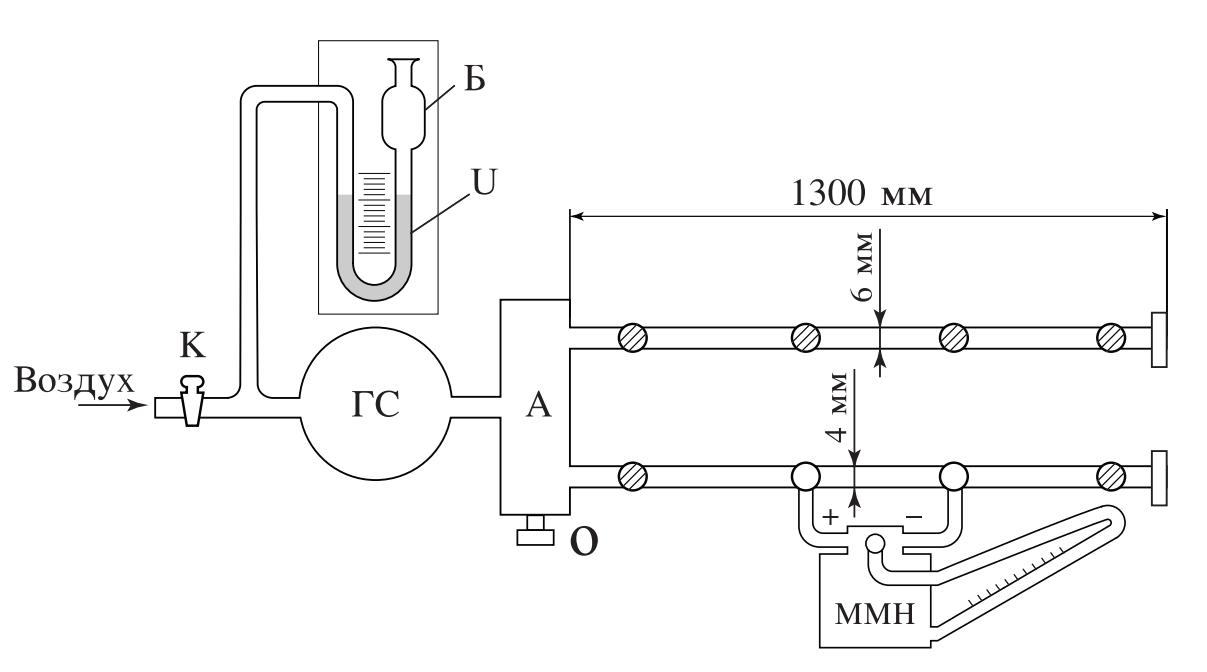
\includegraphics[scale=0.7]{asd.png}
Выразим искомую вязкость через коэффициент наклона прямой $\alpha$
$$h=\eta*\frac{8l}{\pi r^4K*8,80665}Q=\alpha Q$$
$$\eta = \frac{\pi r^4 K*9,80665 \alpha}{8l}$$
$l=(50,0\pm0,1$) cм \\
$r=(1,95\pm0,03$) cм \\
$\epsilon_\eta = \sqrt{4\epsilon_r^2+\epsilon_\alpha^2+\epsilon_l^2}=0,03$\\
\begin{tabular}{|c|}
\hline 
$\eta =(1,61\pm0,05)*10^{-5}$ кг*м/с \\ 
\hline 
\end{tabular} 
\ \\
\ \\
\ \\
Из графика видно, что ламинарный режим переходит в турбулентный на значениях $(8-9)*10^2 \ $м$^3$/с
$$Re=\frac{Qr\rho}{S\eta}$$
$Re=(980-1100)$
\ \\
\ \\
\begin{tabular}{|c|}
\hline 
$Re=1040\pm60$\\ 
\hline 
\end{tabular}
\ \\
\ \\
При расходе, заведомо обеспечивающем ламинарность потока измерим распределение давления вдоль трубки:\\
\ \\
\begin{tabular}{|c|c|c|c|c|c|}
\hline 
l, см & 0 & 10,5 & 40,5 & 80,5 & 130,5 \\ 
\hline 
h, дел & 0 & 16 & 36 & 59 & 88 \\ 
\hline 
\end{tabular} 

\ \ Построим график зависимости давления от расстояния и по прямолинейному участку графика определим вязкость $\mu$: \\
\ \\
\ \\
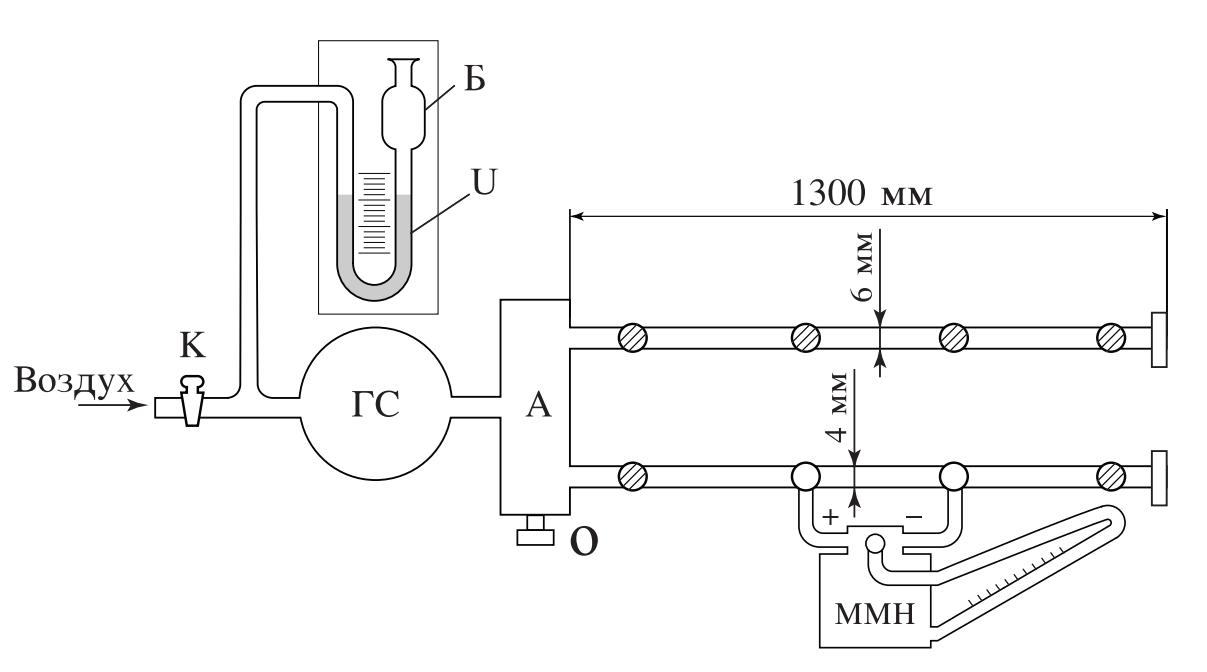
\includegraphics[scale=0.53]{asd.png}
\newpage
Из графика видно, что установление потока происходит еще на 1-ом участке длиной 10,5 см. Теоретические расчеты дали длину установления порядка 40 см. То есть оценка, полученная по формуле, гораздо более грубая, чем результат, который мы наблюдаем в эксперименте.
\ \\
\ \\
\indent Для всех трубок проведем измерения зависимости Q от P и обработаем их по формуле 
$$\frac{8l\eta Q}{\pi(P_1-P_2)}=r^n$$
$$\ln(\frac{8l\eta Q}{\pi(P_1-P_2)})=n\ln r$$
$$\ln1=n\ln2$$
\indent Таблица измерений: \\
\begin{tabular}{|c|c|c|c|}
\hline 
r, см & 1,50 & 1,95 & 2,95 \\ 
\hline 
l, см & 30 & 50 & 50 \\ 
\hline 
h, дел & 11 & 16 & 5 \\ 
\hline 
V нач, л & 4,0 & 4,6 & 1,7 \\ 
\hline 
V конеч, л & 5,3 & 6,8 & 3,0 \\ 
\hline 
t, с & 46 & 89 & 42 \\ 
\hline 
q*10$^2$, л/c & 2,17 & 2,47 & 3,10 \\ 
\hline 
ln1 & -25,65 & -24,85 & -23,46 \\ 
\hline 
ln2 & -6,5 & -6,24 & -5,83 \\ 
\hline 
\end{tabular}
\ \\
\ \\
\ \\
$\Delta ln1 = \sqrt{\epsilon_Q^2+\epsilon_\eta^2+\epsilon_{2h}^2}=0,05$\\
$\Delta ln2 = \epsilon_r$
\ \\
Построим график зависимости $Q = f(l)$:
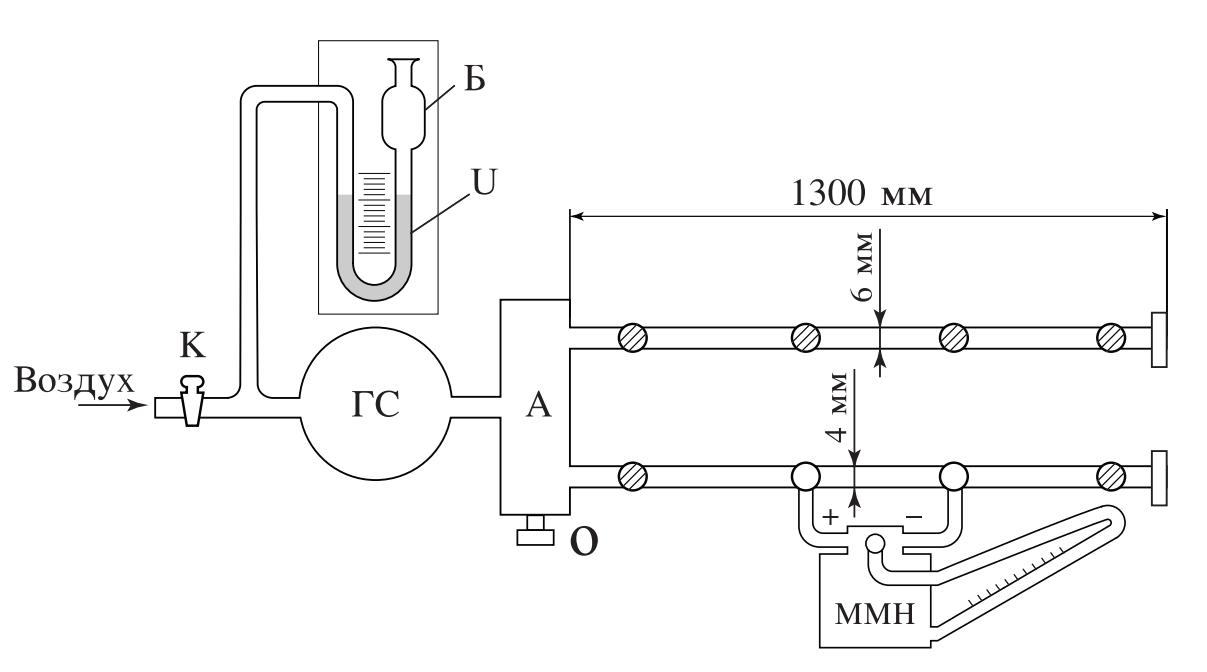
\includegraphics[scale=0.55]{asd.png}
\ \\
\begin{tabular}{|c|}
\hline 
$n=3,97\pm0,05$ \\ 
\hline 
\end{tabular} 
\\
\\
Результат, прекрасно сходящийся с формулой Пуазейля 
\end{document}